\hypertarget{restructuring-existing-code}{%
\section{Restructuring existing
code}\label{restructuring-existing-code}}

\begin{tcolorbox}[colback=blue!5!white,colframe=blue!75!black]
You

\begin{itemize}
\tightlist
\item
  know and can explain the reengineering life cycle
\item
  understand and can apply principles of code restructuring
\item
  know and can apply the OO reverse engineering and reengineering
  patterns
\end{itemize}
\end{tcolorbox}

\hypertarget{software-evolution}{%
\subsection{Software Evolution}\label{software-evolution}}

New or changing requirements will gradually degrade original design. And
sometimes there's literally no time to do a proper refactoring for such
changes. In this cases, it's also possible to do a hack to meet the
deadline, but you also need to invest time in future to do the
implemenation properly.


\paragraph{Technical Dept:} Means that you have to invest even more time in future for a quick \& dirty hack right now. Because you mess up your design with that and you will pay for degrading it in invest more time in the future to bring it back to your good design.


\hypertarget{terminology}{%
\subsubsection{Terminology}\label{terminology}}

\begin{itemize}
\tightlist
\item
  \textbf{Forward Engineering} is the traditional process of moving from
  high-level abstractions and logical, implementation-independent
  designs to the physical implementation of a system.
\item
  \textbf{Reverse Engineering} is the process of analyzing a subject
  system to identify the system's components and their
  interrelationships and create representations of the system in another
  form or at a higher level of abstraction.
\item
  \textbf{Reengineering} is the examination and alteration of a subject
  system to reconstitute it in a new form and the subsequent
  implementation of the new form.
\end{itemize}

\hypertarget{goals-of-reverse-engineering}{%
\subsubsection{Goals of Reverse
Engineering}\label{goals-of-reverse-engineering}}

\begin{itemize}
\tightlist
\item
  Cope with complexity

  \begin{itemize}
  \tightlist
  \item
    need techniques to understand large, complex systems
  \end{itemize}
\item
  Recover lost information

  \begin{itemize}
  \tightlist
  \item
    extract what changes have been made and why
  \end{itemize}
\item
  Generate alternative views

  \begin{itemize}
  \tightlist
  \item
    automatically generate different ways to view systems
  \end{itemize}
\item
  Detect side effects

  \begin{itemize}
  \tightlist
  \item
    help understand ramifications (Verzweigung) of changes
  \end{itemize}
\item
  Synthesize higher abstractions

  \begin{itemize}
  \tightlist
  \item
    identify latent abstractions in software
  \end{itemize}
\item
  Facilitate reuse

  \begin{itemize}
  \tightlist
  \item
    detect candidate reusable artifacts and components
  \end{itemize}
\end{itemize}


\hypertarget{goals-of-reengineering}{%
\subsubsection{Goals of Reengineering}\label{goals-of-reengineering}}
\begin{itemize}
    \item Unboundling
    \subitem Split Monolithiy system into separat parts
    \item Performance
    \subitem first do it, then do it right, then do it fast.
    \item Port to other Platform
    \subitem Point out dependency of the architecture
    \item Design Extraction
    \subitem To improve maintainability, portability etc.
\end{itemize}


\hypertarget{the-reengineering-life-cycle}{%
\subsubsection{The reengineering
life-cycle}\label{the-reengineering-life-cycle}}

\begin{figure}[H]
\centering
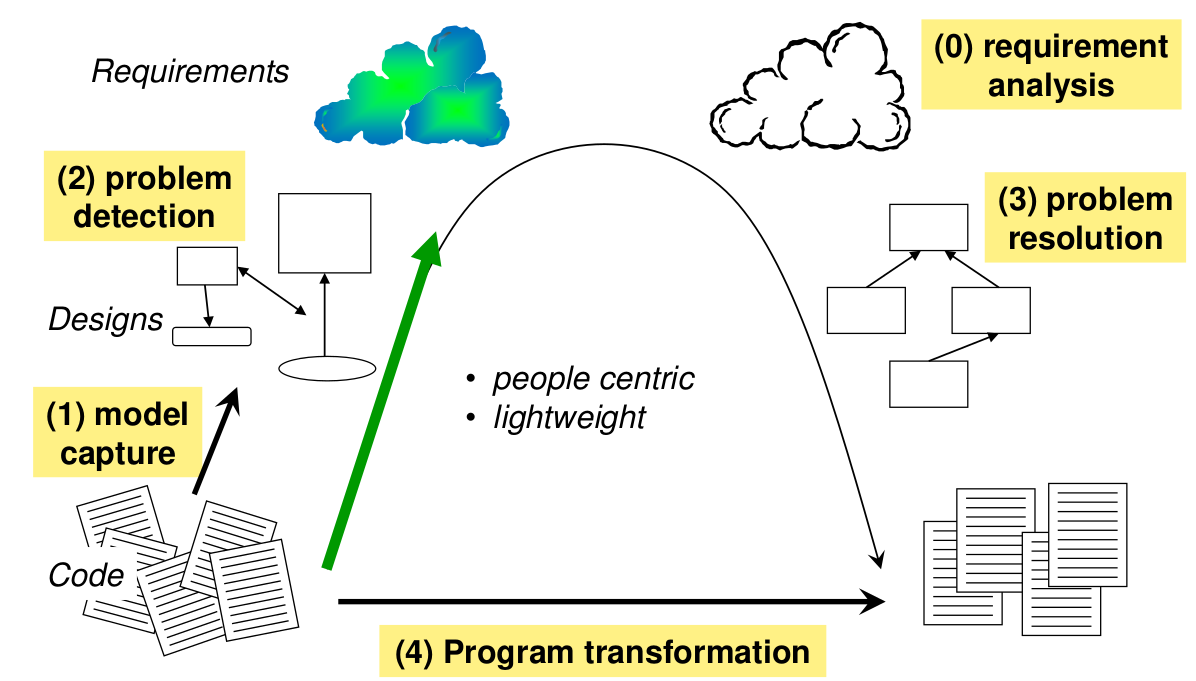
\includegraphics[width=0.5\textwidth]{figures/reengineeringLifecycle.png}
\caption{The Reengineering Life-Cycle}
\end{figure}

\begin{itemize}
\tightlist
\item
  The reverse engineering part is about the understanding the current
  software
\item
  The reengineering part is about to change the existing software and
  create a new one
\end{itemize}

\hypertarget{reverse-engineering-reengineering-patterns}{%
\subsection{Reverse Engineering / Reengineering
Patterns}\label{reverse-engineering-reengineering-patterns}}

\begin{figure}[H]
\centering
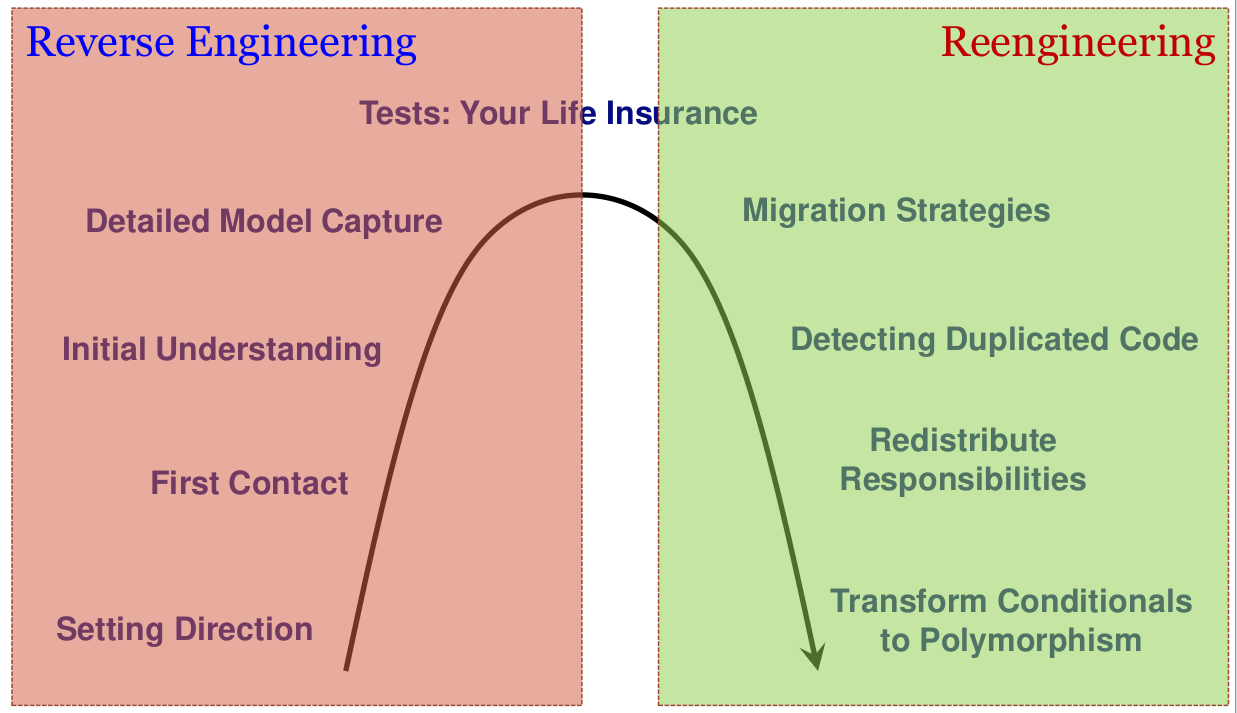
\includegraphics[width=0.5\textwidth]{figures/rePatterns.png}
\caption{Patterns}
\end{figure}


\subsection{Reverse Engineering Pattern}

\hypertarget{settings-direction}{%
\subsubsection{Settings Direction}\label{settings-direction}}
\begin{figure}[H]
\centering
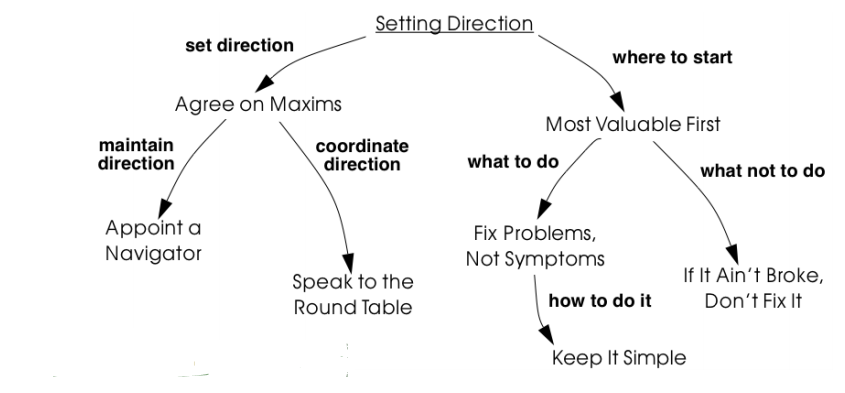
\includegraphics[width=0.5\textwidth]{figures/ReverseEngineering.PNG}
\caption{Setting Direction}
\end{figure}

\begin{itemize}
\tightlist
\item
    Important things first.
\item
  The legacy system will pull you towards a certain architecture that
  may not be the best for the future of the system
\item
  You will detect many problems with the legacy software, and it will be
  hard to set priorities.
\item
  This pattern is about to define the direction to go and decide what to
  change and priorize what
\end{itemize}

\hypertarget{strategies}{%
\paragraph{Strategies}\label{strategies}}

\begin{itemize}
\tightlist
\item
  Agree on Maxims

  \begin{itemize}
  \tightlist
  \item
    How do you establish a common sense of purpose in a team?
  \item
    Agree on specific modules / parts of a system and formulate a clear
    goal
  \end{itemize}
\item
  Most Valuable First

  \begin{itemize}
  \tightlist
  \item
    Which problems should you focus on first?
  \item
    Work on the aspects that are most valuable to your customer or your
    company.
  \end{itemize}
\end{itemize}

\hypertarget{first-contact}{%
\subsubsection{First Contact}\label{first-contact}}

You need to get familiar now with the software system.
Important is that you set boundarys. It is easy to get lost in code. One should also split the system into managable parts and then go through it this has the advantage that you can go over it in a team.

\begin{figure}[H]
\centering
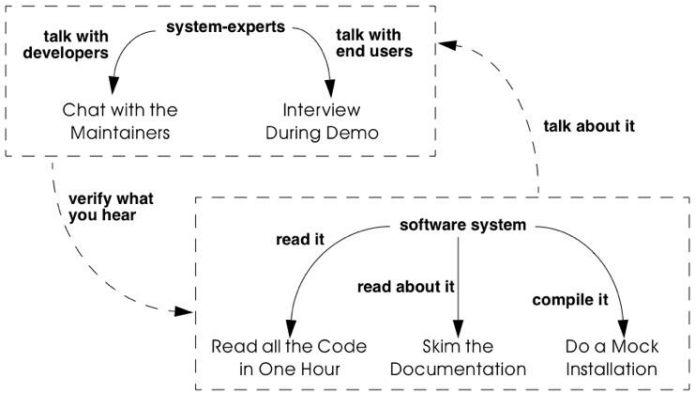
\includegraphics[width=0.5\textwidth]{figures/FirstContact.PNG}
\caption{First Contact Pattern}
\end{figure}



\begin{itemize}
\tightlist
\item
  talk with existing developers
\item
  talk with end users
\item
  verify what you hear in the code

  \begin{itemize}
  \tightlist
  \item
    read the code
  \item
    read the documentation
  \item
    compile it
  \end{itemize}
  \item Read all the code in one Hour
\end{itemize}



\subsubsection{Initial Understanding}
In this steps it is about verifying your knowledge about the code. It is best to develop a hypotheses and then discuss with a native. Also analyze the Databse schema and figure out the structure of it. Always document your findings for the rest of the team.
\begin{figure}[H]
\centering
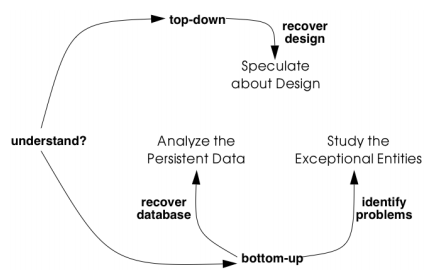
\includegraphics[width=0.5\textwidth]{figures/InitialUnderstanding.PNG}
\caption{Initial Understanding Pattern}
\end{figure}































\subsubsection{Detailed Model Capture}
Deepen your understanding of the source code. You can easily write comment into the source files. Start to iteratively refactor a part of the software to validate your understanding. Stepping trough the execution always helps to see the interaction between objects. Writes Tests to understand what happens.
\begin{figure}[H]
\centering
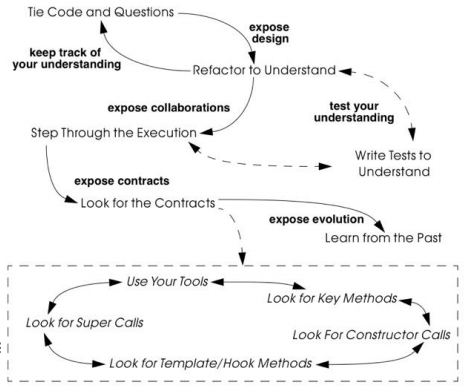
\includegraphics[width=0.5\textwidth]{figures/ModelCapture.PNG}
\caption{Model Capture Pattern}
\end{figure}




























\subsection{Reengineering Pattern}
\hypertarget{redistribute-responsibilities}{%
\subsubsection{Redistribute
Responsibilities}\label{redistribute-responsibilities}}

\begin{itemize}
\tightlist
\item
  The Law of Demeter (loose coupling)

  \begin{itemize}
  \tightlist
  \item
    Each unit should have only limited knowledge about other units: only
    units ``closely'' related to the current unit.
  \item
    Each unit should only talk to its friends; don't talk to strangers.
  \item
    Only talk to your immediate friends.
  \end{itemize}
\item
  Eliminate Navigation Code

  \begin{itemize}
  \tightlist
  \item
    Navigation Code leads to tight Coupling
  \end{itemize}
\item
  Split Up God Class
\item
  Move Behavior Close to Data
\end{itemize}

\clearpage